%\section[Projected Equations of Motion (PEOM) Method for Semiconductor-Metal Composites]{Projected Equations of Motion (PEOM) Method for\\ {Semiconductor-Metal} Composites}\label{sec:peom}
\section{Projected Equations of Motion (PEOM) Method for\\ {Semiconductor-Metal} Composites}\label{sec:peom}

The efficiency of a PV device is largely determined by its ability to absorb
light. We mentioned in \cref{sec:light_2d} that the performance of 2D,
TMD-based solar cells may be improved by depositing MNPs on the TMD monolayer.
In the presence of light, the MNPs enhance the field near the monolayer which
in turn increases its light absorption.

The absorption in the monolayer may be obtained theoretically using the methods
described in \cref{sec:background_theory}. For example, to calculate the
absorption in a monolayer of \ce{MoS2}, one would first perform a DFT calculation on
a unit cell (containing three atoms) to determine the ground state electronic
configuration. A linear response TDDFT calculation could then be carried out
and the optical absorption spectrum obtained. Such calculations are routine and
can be easily completed on a modern desktop computer in a relatively short
period of time. Suppose we now wish to perform a similar calculation for an
\ce{MoS2} monolayer decorated with gold nanoparticles of diameter
\SI{15}{\nano\metre}, similar to the system studied experimentally in
Ref.~\cite{Lin2013}. In this case, one
must construct a supercell containing around \num{50000} times more atoms and
having a volume greater than \num{100000} times that of the original unit
cell of the bare \ce{MoS2} monolayer. Such a calculation at the DFT level would
prove extremely demanding: even with a
linearly scaling code running on many cores of a supercomputer, the
boundaries on computational resources are being pushed if not exceeded.
Moreover, the calculation becomes infeasible if one
wishes to model excitonic effects using, for example, the Bethe-Salpeter
Equation as described in
~\cref{sec:background_theory}.

For this system, however, we are interested primarily with the optical response
of the \ce{MoS2} monolayer as it is the `active' component of the PV device. The MNP
on the other hand contributes just to modify the optical properties of the
monolayer. Due to the large difference in scale of the MNP compared to the
monolayer (in terms of the unit cells required for the DFT calculations), it
may then be appropriate to model the MNP on a level of theory less
computationally demanding than DFT and to couple the dynamics to those of the
monolayer by some effective method. 

Indeed, similar problems occur in other areas of computational chemistry and
various hybrid methods have been used to great effect over the past few
decades. For example, the quantum mechanics/molecular mechanics (QM/MM)
approach has been widely applied to study chemical reactions in large systems.
In the QM/MM method, the larger environment (e.g. a solvent) is treated on the
basis of classical molecular mechanics while the smaller system of interest
(e.g. a molecule) is treated using a quantum approach (e.g. DFT). The two
systems can then be coupled via force fields or electrostatically as in the
polarizable continuum model.

In Ref.~\cite{Zhang2006} a method is developed for modelling the interaction
between a semiconducting quantum dot (SQD) and an MNP under illumination. In
this case, the SQD is treated as a two-level atomic-like system using the
density matrix formalism of quantum mechanics while the MNP is modelled using
classical electrodynamics. The dynamics of the two systems are then coupled
through the externally applied field using a dipole-dipole approximation. The
dynamics of this hybrid complex can be solved analytically within the so-called
rotating wave approximation (RWA) as described in detail in \cref{app:sqd-mnp}. This
analytical solution is valid provided the applied field is a slowly-varying
monochromatic pulse of frequency close to the frequency gap of the SQD.
Moreover, the optical response function of the MNP is assumed to be much
broader than that of the SQD which is inherently narrow due to its two-level
nature and relatively long dephasing times. As it stands, the solution will not
hold for ultrafast pulse excitation which is an area of current interest for
such systems. Moreover, if the SQD is replaced with a semiconducting monolayer,
the two-level quantum description will not suffice and the profile of the
MNP response function can no longer be considered `broad'. Therefore, the method
should be generalised to lift the restrictive approximations commonly used,
giving rise to the proposed project equations of motion (PEOM) approach
described in this section. 

\begin{figure}[ht]
    \centering
    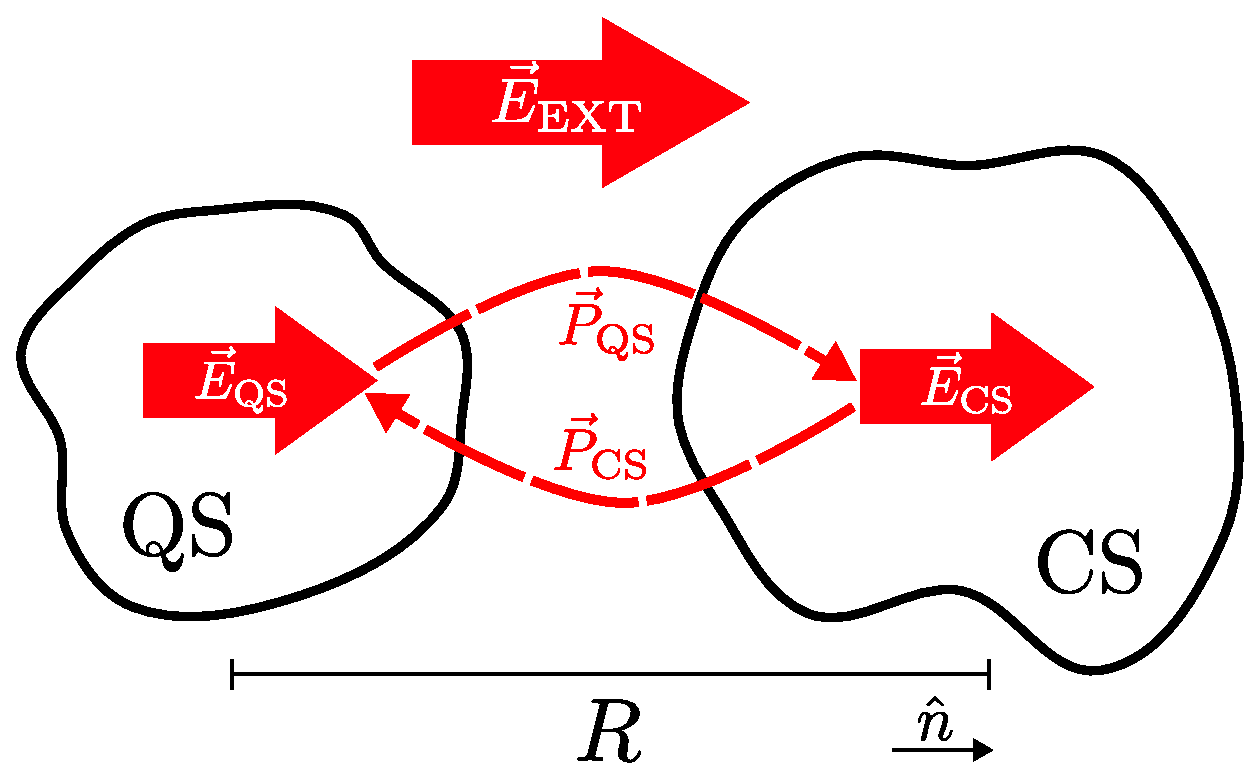
\includegraphics[width=0.6\columnwidth]{img/qs-cs.eps}
    \caption{Schematic diagram showing the dipole-dipole interaction between a
        QS and a CS, separated by a distance $R$.  When an external field,
        $\veext$, is applied, a dipole moment, $\vpqs$, is induced in the QS,
        generating a field. The CS thus experiences this dipole field in
        addition to the external field, and we denote the total field felt by
        the CS as $\vecs$. Similarly, due to $\vecs$, a dipole field is
        generated in the CS which is in turn felt by the QS in addition to
        $\veext$, and we denote the total field felt by the QS as $\veqs$. In
    this way, the QS and CS dynamics are coupled through the external field.}
    \label{fig:qs-cs}
\end{figure}

\note{[Would the terms ``primary system'' and ``auxiliary system''
describe the setup better?]} In order to introduce the PEOM method, 
we consider a general composite comprising two, isolated subsystems in a vacuum:
a larger system to be treated
classically---the classical system (CS)---and a smaller system of interest to
be treated on the basis of quantum mechanics---the quantum system (QS). For
example, in the semiconducting monolayer-MNP system, the monolayer would be the
QS and the MNP the CS. The QS and CS shall be separated by some distance, $R$.
An external field, $\veext(t)$, is applied which induces a dipole-dipole
interaction between the two systems as described in \cref{fig:qs-cs}.
To simplify the
notation, we assume that the QS and CS are isotropic media. For the
generalization to the anisotropic case see \cref{app:anis}.
We write
$\veext(t)\equiv\eext(t)\ve$ and denote the unit vector pointing along the
line separating the centres of the systems as $\hat n$. The fields felt by
the QS and CS are then,
respectively~\cite{jackson_classical_1962,schmitt_preparation_1999,zhang_semiconductor-metal_2006},
\note{(note that I've removed the background dielectric constant, $\epsb$, as I
only ever use a vacuum and it simplifies notation.)}
%
\begin{subequations}
    \begin{align}
        \veqs(t) &= \eext(t)\ve + \frac{\pcs(t)}{\epsb R^3}\g \ , \label{eq:eqs}\\
        \vecs(t) &= \eext(t)\ve + \frac{\pqs(t)}{\epsb R^3}\g \ , \label{eq:ecs}
    \end{align}
    \label{eq:fields1}
\end{subequations}
%
where $\pcs(t)$ ($\pqs(t)$) is the total dipole moment of
the CS (QS), and
%
\begin{equation}
    \g=3\hat n\left( \ve \cdot \hat n \right) - \ve \ .
    \label{eq:g_def}
\end{equation}
%
\note{Is this actually correct? I can see that if $\hat n$ is parallel or
perpendicular to $\hat e$ then yes, but what if it's at 45 degrees? Will there
be a dipole along $\hat e$ and $\hat n$ both?\ldots}

The time-dependent dipole moment of the QS, $\pqs(t)$, can be
obtained, e.g., using the methods outlined in Section REF. In general, it is
found by solving some equations of motion, whether they be from the density matrix
master equation (Eq. REF), or the real-time Bethe-Salpeter equation (Eq. REF),
although the theory presented here is independent of the chosen method.

For the CS, rather than calculate the dipole moment explicitly by solving EOMs
from quantum theory (or even from classical electrodynamics), we assume that
its frequency dependent polarizability, $\alpha(\omega)$, is already known.
This may have been previously obtained, however, from \textit{ab-initio}
calculations similar to the QS, or from experimental data or classical
approximations.  Its dipole moment can then be described (in the linear
response regime) via~\footnote{Gaussian units are assumed throughout this
    thesis \note{--THIS SHOULD GO AT THE START SOMEWHERE INSTEAD.}}
%
\begin{equation}
    \vpcs(\omega) = \epsb  \alpha(\omega)\vecs(\omega) \ .
    \label{eq:pcs_omega}
\end{equation}
%
In the time domain, however, the dipole moment
is written in terms of the response function $\alpha(t)$, as
%
\begin{equation}
    \vpcs(t) = \epsb \int_{-\infty}^{t}\alpha(t-t')\vecs(t')dt' \ .
    \label{eq:P_2}
\end{equation}
%
Now, the EOMs that determine $\vpqs(t)$ depend on $\veqs(t)$ which in turn
depends on $\vpcs(t)$ from \cref{eq:eqs}. They are generally solved
using an iterative algorithm, such as the fourth-order Runge-Kutta method (see
\cref{app:runge-kutta} \note{--not sure whether it's necessary to include this
in the appendix\ldots}), where the time domain is split into a set of discrete points.
However, computing the integral in Eq.~\eqref{eq:P_2} at each time-step in the
solution is cumbersome and the values of $\vecs(t)$ and $\alpha(t)$ for each
time-step must be held in memory which may not be feasible for long
simulations.  Moreover, while $\alpha(\omega)$ is known beforehand, $\alpha(t)$
is not and would have to be calculated using, e.g., a discrete fourier
transform. In this case one would have to ensure a sufficiently large
(\note{small?}) time-resolution of the transform in order to match the
time-step in the algorithm used to solve the quantum EOMs. However, the
resolution is limited to whatever data is available for $\alpha(\omega)$.
\note{ Not sure if this last part is necessary, or too confusing. Also,
would this method actually work? I would guess a very small time-step would be
needed\ldots }

In Ref.~\cite{stella_generalized_2014}, a method (originally devised for memory
kernels in the Generalised Langevin Equation) is presented for avoiding the
memory-dependent time-convolution inherent in \cref{eq:P_2}. Inspired by this,
we introduce $N$ complex auxiliary degrees of freedom, $\{\vs_k(t)\}$ which
satisfy the following projected equations of motion (PEOMs)
%
\begin{equation}\label{eq:s_EOM}
    \dot{\vs}_k = -\left( \gamma_k + \imagn\omega_k \right)\vs_k + \imagn\epsb
    \vecs(t)\ \quad \text{for }k=1,2,\ldots,N \
    .
\end{equation}
%
We then state that $\vpcs(t)$ can be written as
%
\begin{equation}\label{eq:P_2_approx}
    \vpcs(t) \approx \sum_{k=1}^{N} c_k \real{\vs_k(t)} \ ,
\end{equation}
%
so that the memory-dependent integral in Eq.~\eqref{eq:P_2} is replaced with an
expansion over the functions $\vs_k$ found by solving the differential
equations in Eq.~\eqref{eq:s_EOM}. As these differential equations no longer
contain a time-convolution (i.e., they are ``memoryless''), they can be
efficiently integrated using, e.g., the same iterative algorithm as for the QS. 
Therefore, the QS EOMs and the CS PEOMs can be efficiently solved in a coupled
fashion.
All that
is required is to find suitable values for the (real) parameters $\{c_k,
\gamma_k, \omega_k\}$ in Eq.~\eqref{eq:s_EOM}.
The formal solution of Eq.~\eqref{eq:s_EOM} is
%
\begin{equation}
    \vs_k(t) = \epsb \int_{-\infty}^{t}\imagn\ e^{-\left( \gamma_k + \imagn\omega_k
    \right)\left( t-t' \right)} \vecs (t') dt' \ .
    \label{eq:s_k}
\end{equation}
%
Substituting the real part of Eq.~\eqref{eq:s_k} into Eq.~\eqref{eq:P_2_approx} and
rearranging yields
%
\begin{equation}
    \vpcs(t) \approx \epsb
    \int_{-\infty}^{t} 
    \left( 
        \sum_{k=1}^{N} c_k e^{-\gamma_k (t-t')}\sin[\omega_k(t-t')]
    \right) 
    \vecs(t') dt' \ ,
\end{equation}
%
and comparing with Eq.~\eqref{eq:P_2} we see that
%
\begin{equation}
    \alpha(t) \approx 
        \sum_{k=1}^{N} c_k e^{-\gamma_k t}\sin(\omega_k t) \ .
    \label{eq:chi_t}
\end{equation}
%
Taking the Fourier transform of
Eq.~\eqref{eq:chi_t} (using the causality condition) gives
%
\begin{equation}
    \alpha(\omega) \approx \sum_{k=1}^{N}\frac{c_k}{2}
    \left[ \frac{1}{\omega+\omega_k +\imagn\gamma_k}
    -\frac{1}{ \omega-\omega_k +\imagn\gamma_k}\right] \ .
    \label{eq:chi_approx}
\end{equation}
%
Hence, the parameters $\{c_k,\gamma_k,\omega_k\}$ may be found by fitting
the frequency-dependent polarizability of the CS (which is known)
to the functions on the RHS of Eq.~\eqref{eq:chi_approx}
(e.g. using the least squares method\note{--in appendix?}).
